%======================================================================
\subsection{BW-MOD-14 --- Plan: on-canvas editing, first version (23 Oct 2026, approved 24 Oct)}\label{sec:mod14-plan}
%======================================================================

\eref{MOD-14} lets you change a feature where you see it: double-click a face or a feature and a value field and a
drag arrow appear in the 3D view, as in Fusion's press-pull. The first version covers \textbf{Pad and Pocket
(distance), Fillet (radius) and Hole (depth and diameter)}; more features follow the same pattern. The
acceptance stays as written: \emph{pad length, fillet radius and hole depth edited in the view without the task
panel.} The spike below drove a pad from a real drag in this build, from Python only.

\paragraph{Your answers (23 Oct).}
\begin{center}
\small
\begin{tabularx}{\linewidth}{@{}lX@{}}
\toprule
Question & Answer\\
\midrule
First features & Pad/Pocket length, Fillet radius, Hole depth and diameter; more later.\\
Gesture & Double-click a face or a feature $\rightarrow$ a value field and a drag arrow in the 3D view.\\
Undo & One undo step per edit (a whole drag is one step).\\
Basis & FreeCAD~1.1's interactive draggers where they help; find out what Python can reach, and whether
  \code{[BW]} C++ is needed.\\
\bottomrule
\end{tabularx}
\end{center}

\begin{figure}[!htbp]
\centering
\begin{tikzpicture}
  \node[anchor=south west,inner sep=0] (img) at (0,0) {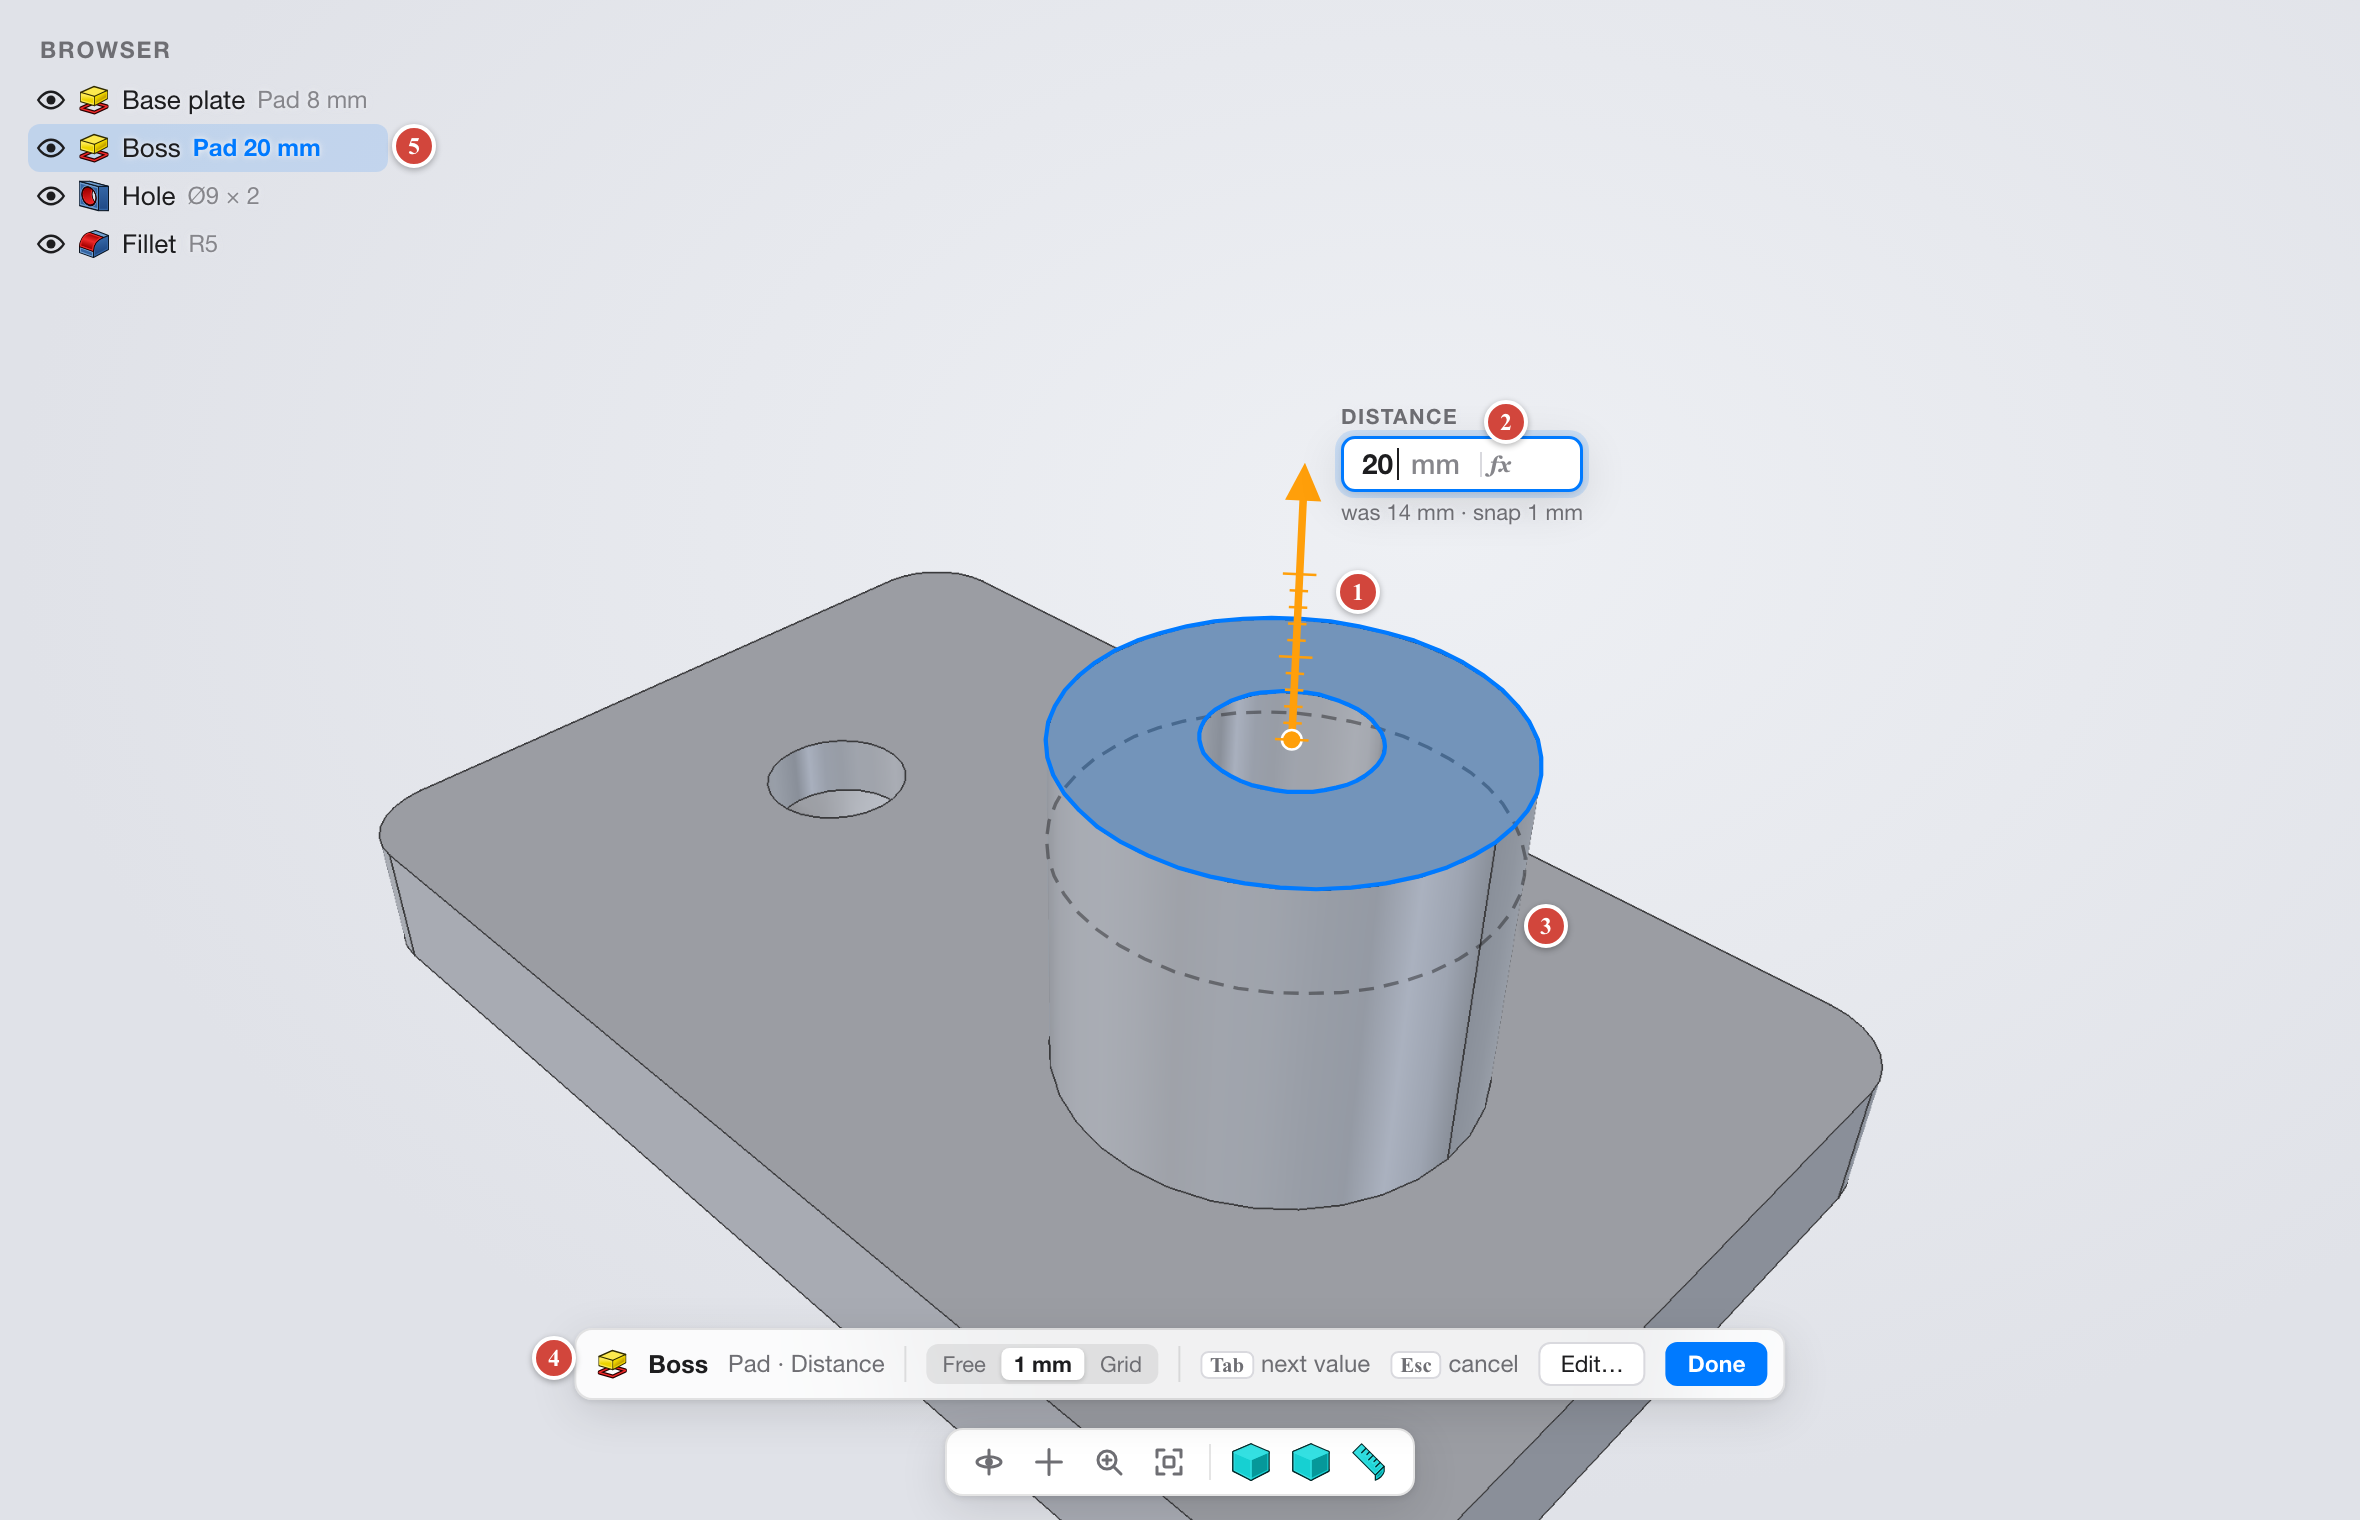
\includegraphics[width=\linewidth]{fig/mod14_pad_notes.png}};
\end{tikzpicture}
\caption{Dragging the Boss pad from 14 to 20\,mm (mock, light). The numbers match the table below.}
\label{fig:mod14-notes}
\end{figure}

\begin{center}
\small
\begin{tabularx}{\linewidth}{@{}cp{3cm}X@{}}
\toprule
\# & Element & Behaviour\\
\midrule
\marker{1} & Drag arrow & Starts on the double-clicked face and points along the feature's direction; accent while
  idle, orange while dragged, with snap ticks along it.\\
\marker{2} & Value field & At the arrow tip; shows the live value, takes typing at once (``20'', ``= Plate.T * 2'',
  ``3/4 in''), Enter applies. Below it: the start value and the snap step.\\
\marker{3} & Face and start & The face being moved is highlighted; a dashed outline shows where it started.\\
\marker{4} & Command bar & What is edited, the snap step (free, 1\,mm, grid), keys, \emph{Edit\ldots} (the full
  task dialog) and \emph{Done}. Sits above the navigation pill.\\
\marker{5} & Browser & The row's summary follows live (``Pad 20 mm''); so does the inspector (\S\ref{sec:uix12-plan}).\\
\bottomrule
\end{tabularx}
\end{center}

\begin{figure}[!htbp]
\centering
\IfFileExists{fig/mod14_pad_dark.png}{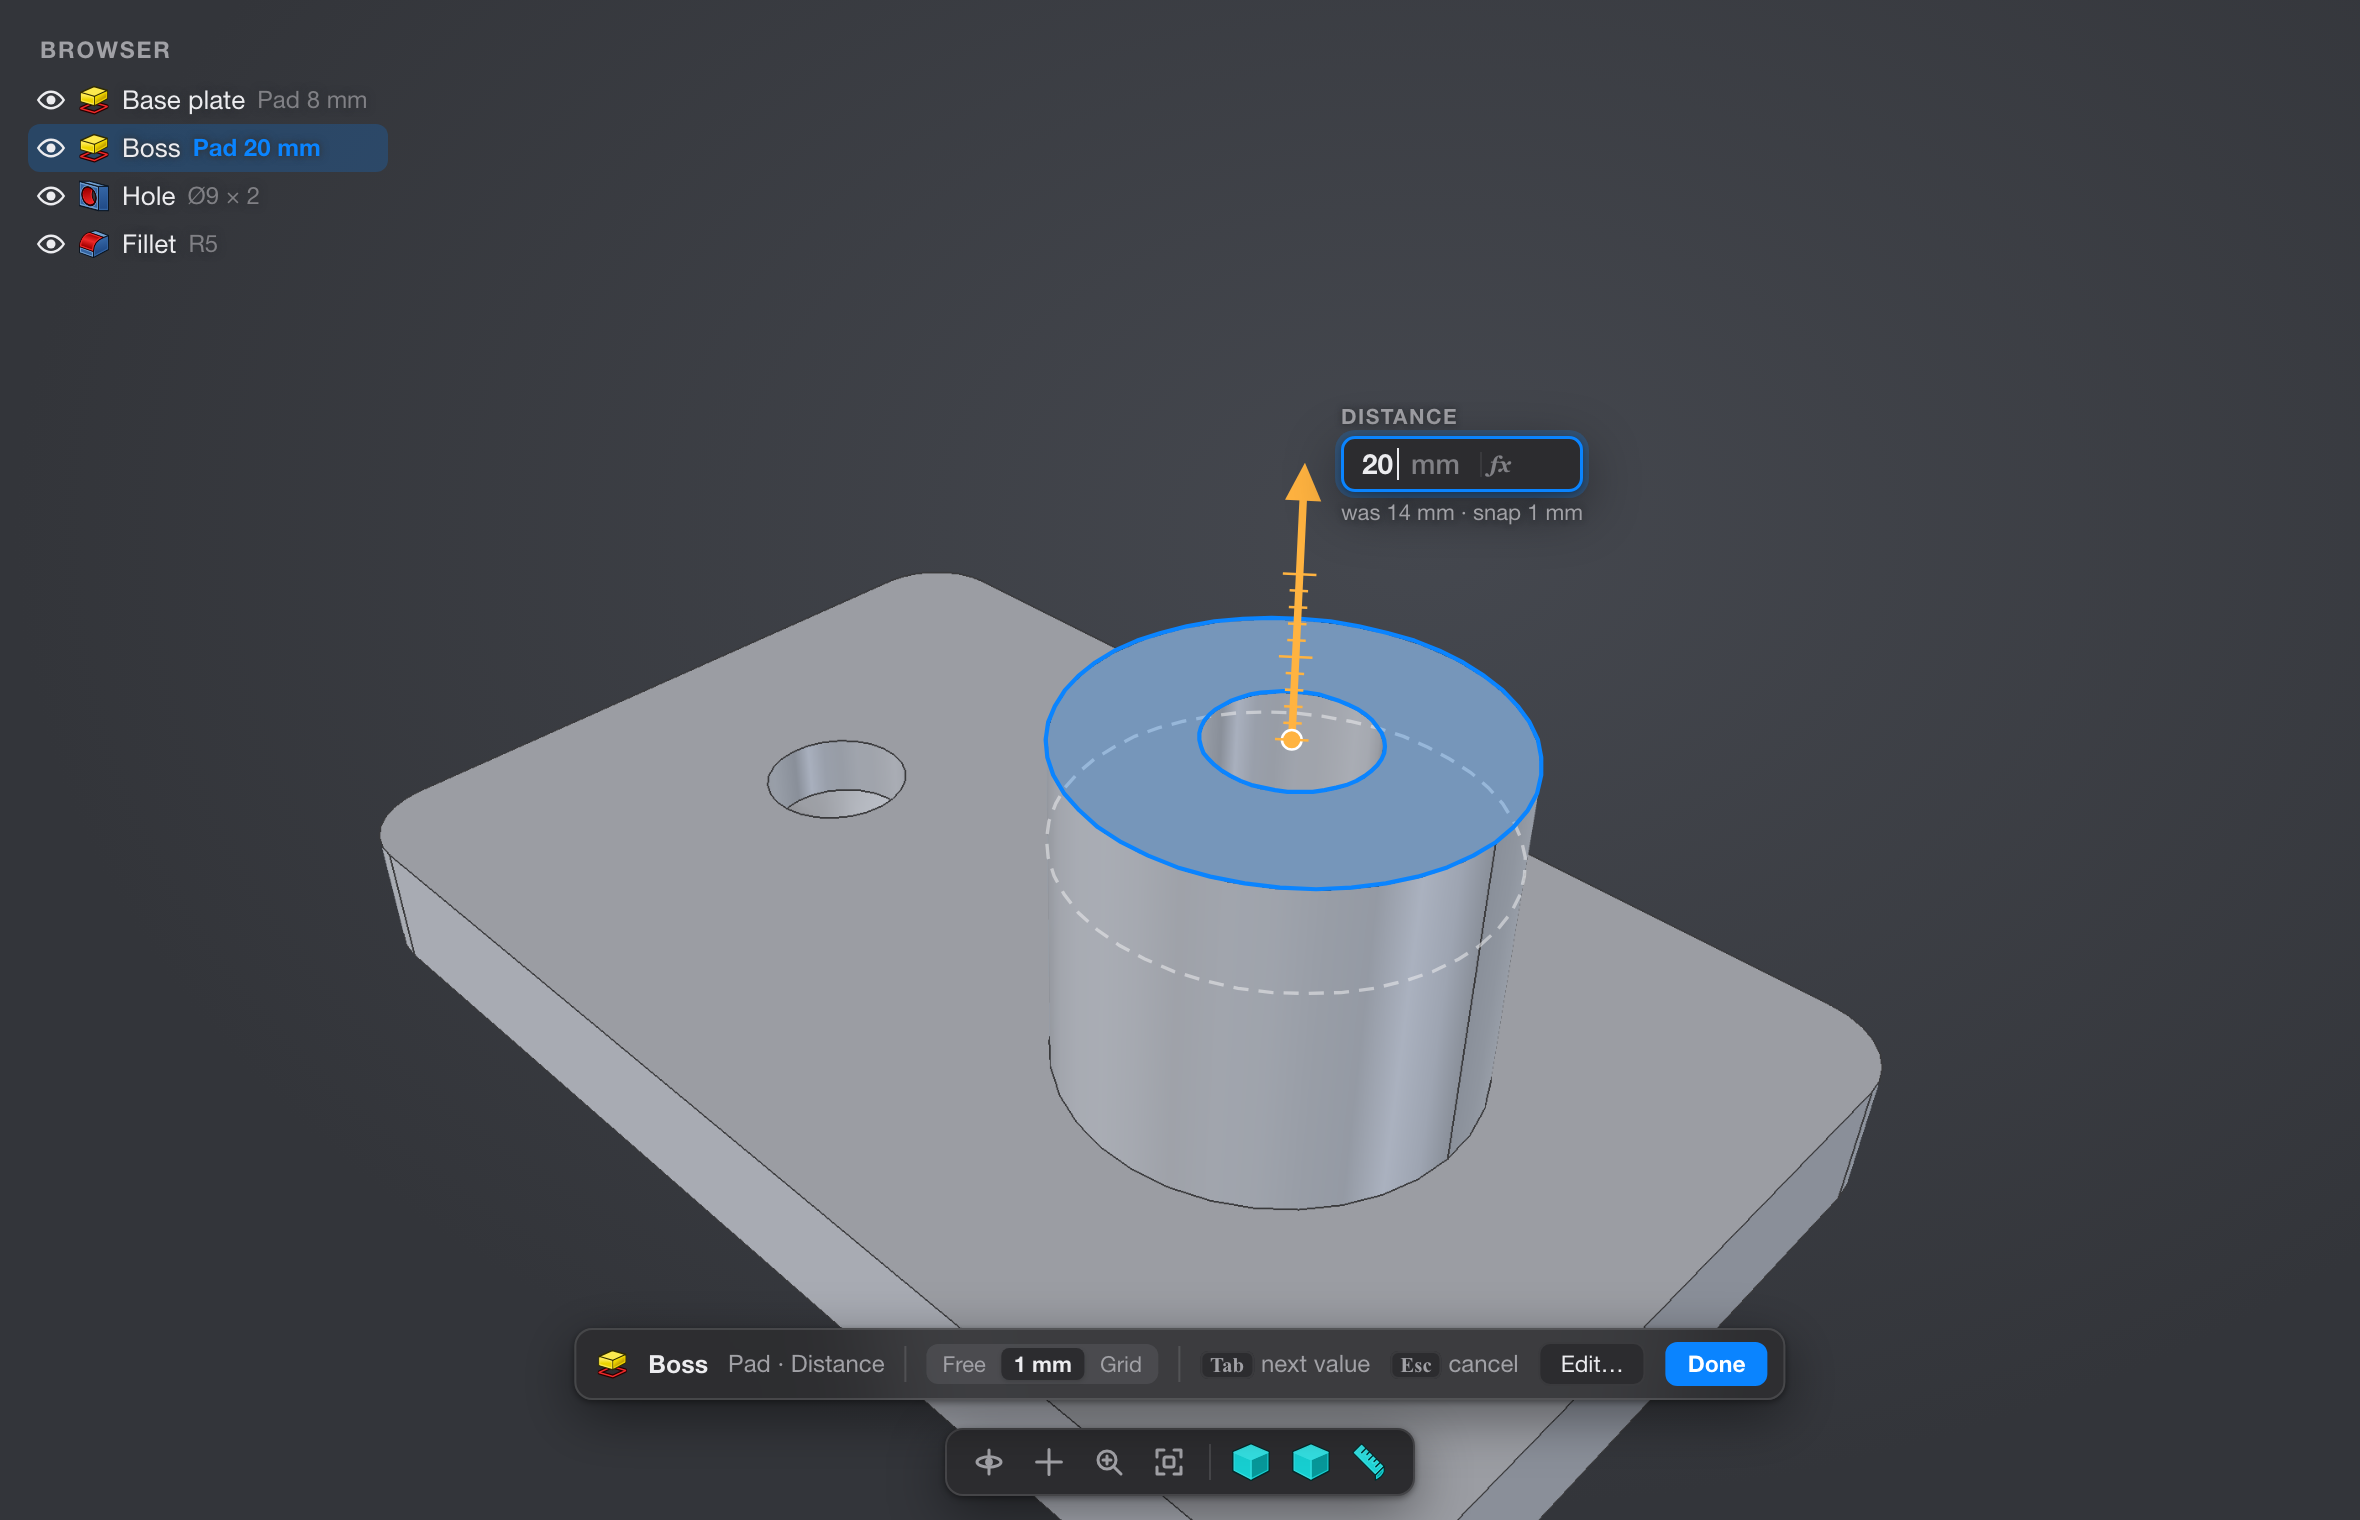
\includegraphics[width=0.75\linewidth]{fig/mod14_pad_dark.png}}{\fbox{mod14\_pad\_dark.png}}
\caption{The same, dark.}
\label{fig:mod14-dark}
\end{figure}

\begin{figure}[!htbp]
\centering
\IfFileExists{fig/mod14_states.png}{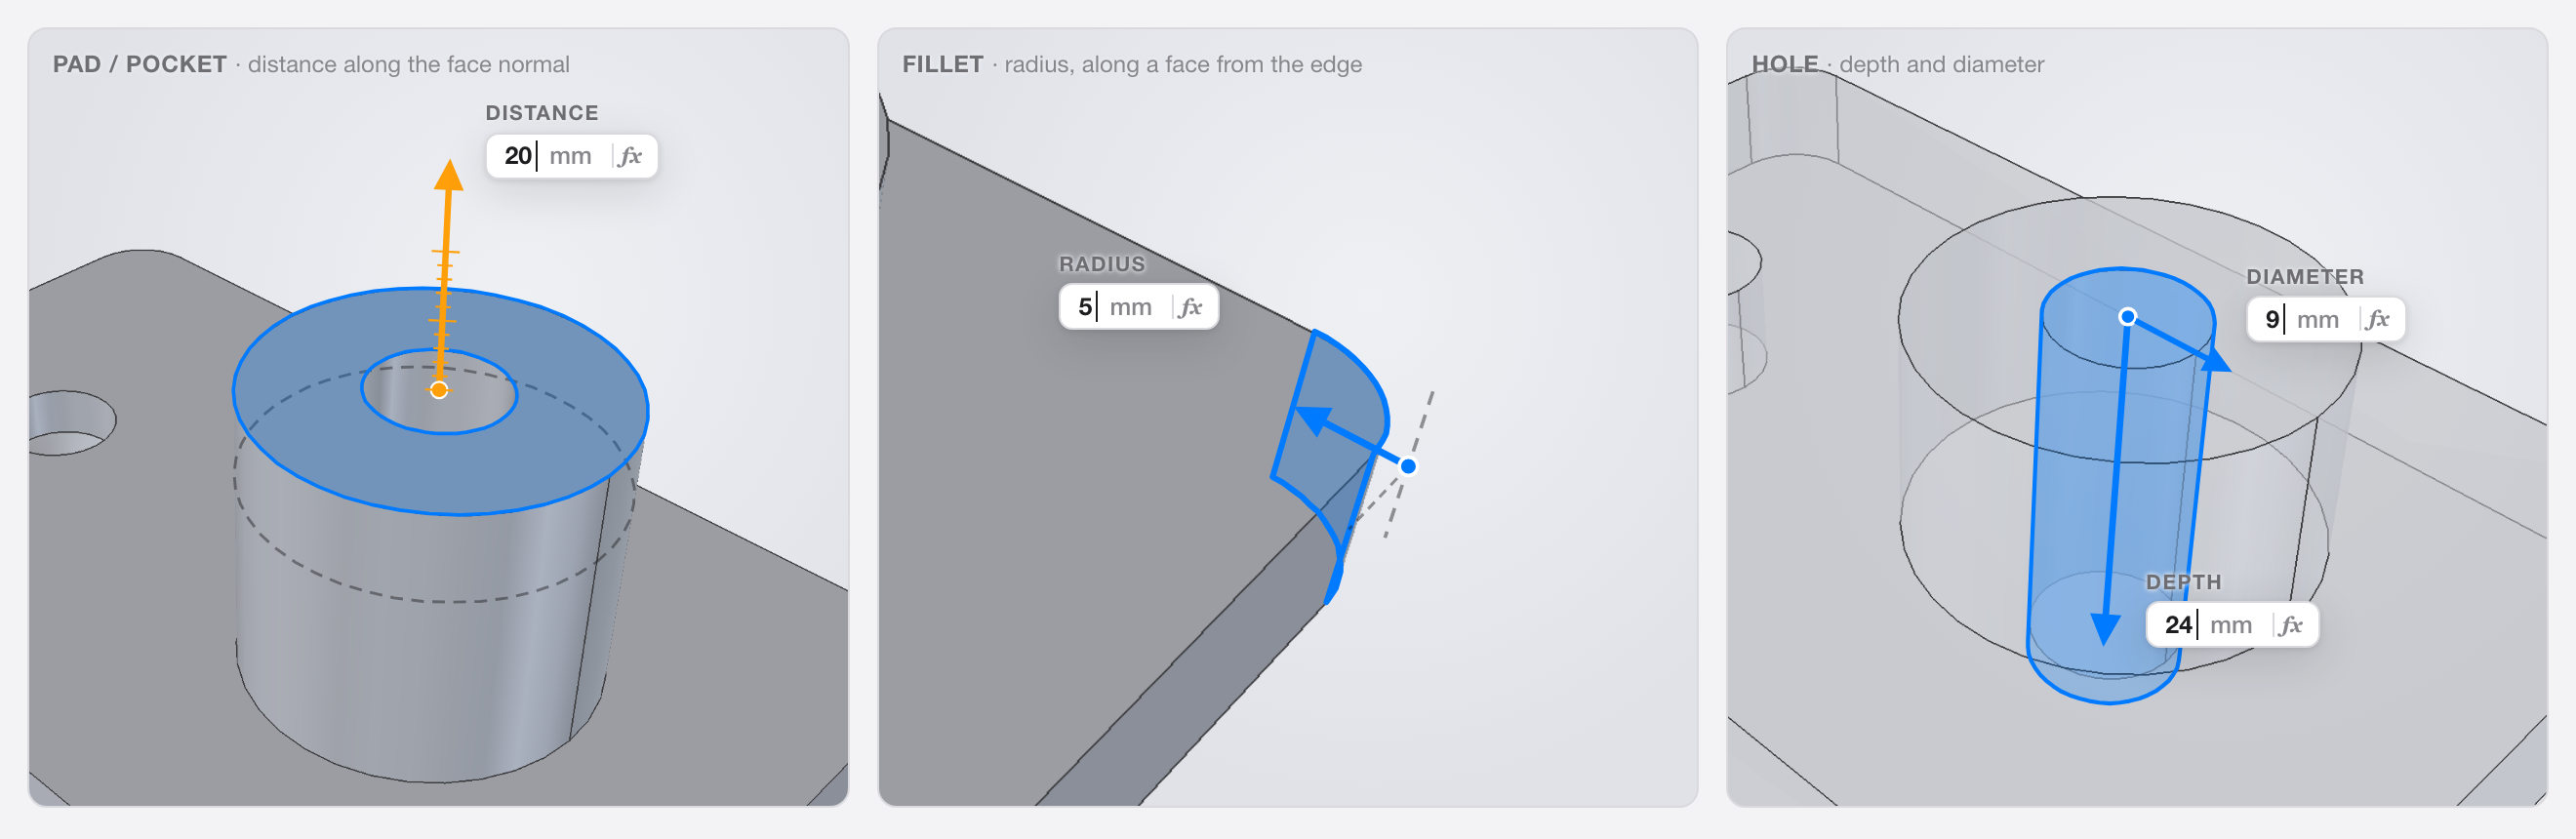
\includegraphics[width=\linewidth]{fig/mod14_states.png}}{\fbox{mod14\_states.png}}
\caption{The three handles of the first version (mock). \emph{Pad/Pocket:} one arrow along the extrusion.
\emph{Fillet:} one arrow on a face next to the filleted edge, from where the sharp edge was (dashed) to where the
fillet meets the face. \emph{Hole:} depth down the axis, diameter out to the rim.}
\label{fig:mod14-states}
\end{figure}

%----------------------------------------------------------------------
\subsubsection*{1. What FreeCAD 1.1 already has, and what Python can reach}

FreeCAD~1.1 added \emph{gizmos}: drag arrows in the view while a feature's task dialog is open
(\file{src/Gui/Inventor/Draggers/}: \code{Gizmo.h}, \code{SoLinearDragger}, \code{SoRotationDragger}).
\begin{center}
\small
\begin{tabularx}{\linewidth}{@{}>{\raggedright\arraybackslash}p{3.4cm}X@{}}
\toprule
Piece & What it is, and from Python\\
\midrule
\code{LinearGizmo}, \code{RotationGizmo}, \code{RadialGizmo}, \code{GizmoContainer} & C++ classes, each tied to one
  \code{QuantitySpinBox} of a task panel; the arrow writes the spin box, the spin box moves the arrow. Used by Pad and
  Pocket (length and taper, both sides), Hole (depth), Fillet (radius, two arrows), Chamfer, Revolution, Helix, Draft
  and Thickness (\code{Task*Parameters::setupGizmos}). \textbf{No Python binding}, and they live only while the task
  dialog is open.\\
Coin node types & \code{SoLinearDraggerContainer}, \code{SoLinearDragger}, \code{SoRotationDragger},
  \code{GizmoContainer}, \ldots{} are registered with Coin (\file{Gui/SoFCDB.cpp}). \textbf{Python can create them by
  type name} and set their fields through pivy (tested below): same arrow, same increments, same look.\\
Placement helpers & \file{Mod/Part/App/GizmoHelper.cpp} (edge mid-point, face normal near an edge, the two faces of
  an edge, the arrow placement for a fillet). C++ only; about 80 lines to port with Part's Python API.\\
Preferences & \code{BaseApp/Preferences/Gui/Gizmos}: \code{EnableGizmos} (on), \code{DelayedGizmoUpdate} (off: the
  value follows the drag live).\\
Colours & Style parameters \code{LinearGizmoBaseColor}, \code{LinearGizmoActiveColor},
  \code{DimensionVisualizerColor} (red, yellow, blue by default). Setting them in the Heuretes FreeCAD theme makes the
  task-panel arrows match ours \verify.\\
\code{View3DInventorPy} & \code{addDraggerCallback(dragger, "addMotionCallback", fn)}, \code{getPointOnViewport},
  \code{getObjectInfo}, \code{getCameraNode}, \code{getSceneGraph}: all a Python editor needs.\\
\bottomrule
\end{tabularx}
\end{center}

\paragraph{The spike (23 Oct).} \file{plan-ui/spike\_canvas.py} built the plate (pad, boss, two holes, four fillets),
put a drag arrow on the boss's top face, a value field over the 3D view, and sent a real mouse drag (press on the
arrow, 12 moves of 8\,px, release) to the view:
\begin{center}
\small
\begin{tabularx}{\linewidth}{@{}lX@{}}
\toprule
Check & Result\\
\midrule
Dragger, pivy & \code{coin.SoTranslate1Dragger} with our own arrow geometry, aligned with the pad direction: works.\\
Dragger, FreeCAD~1.1 & \code{SoLinearDraggerContainer} made by type name, \code{rotation}/\code{translation} and the
  dragger's \code{geometryScale}, \code{translationIncrement} set from Python: \textbf{works}, snapping included.\\
Callbacks & pivy's own \code{SoDragger.addMotionCallback} \textbf{crashes FreeCAD} on the first press (twice, both
  forms). \code{view.addDraggerCallback}, which FreeCAD's Assembly uses, works.\\
Live update & 12 motions $\rightarrow$ 12 recomputes of 19--22\,ms each (the boss, then the hole and fillets after
  it); the arrow and the field follow. Pad 14 $\rightarrow$ 23\,mm.\\
Undo & One transaction from press to release: \textbf{one undo step} (``Drag Boss length''). A typed value is a second
  step; undo returns to 23\,mm.\\
Double-click & An event filter on the 3D viewport receives the double-click; \code{getObjectInfo} at the pointer gives
  \code{Body.Fillet.Face5}. No navigation style uses a left double-click \verify.\\
Recompute times & Headless, same model: boss length 13.9\,ms (the boss alone 1.9\,ms), base plate 6.5\,ms, fillet
  radius 7.8\,ms, hole depth 3.9\,ms.\\
\bottomrule
\end{tabularx}
\end{center}

\begin{figure}[!htbp]
\centering
\IfFileExists{fig/mod14_spike.png}{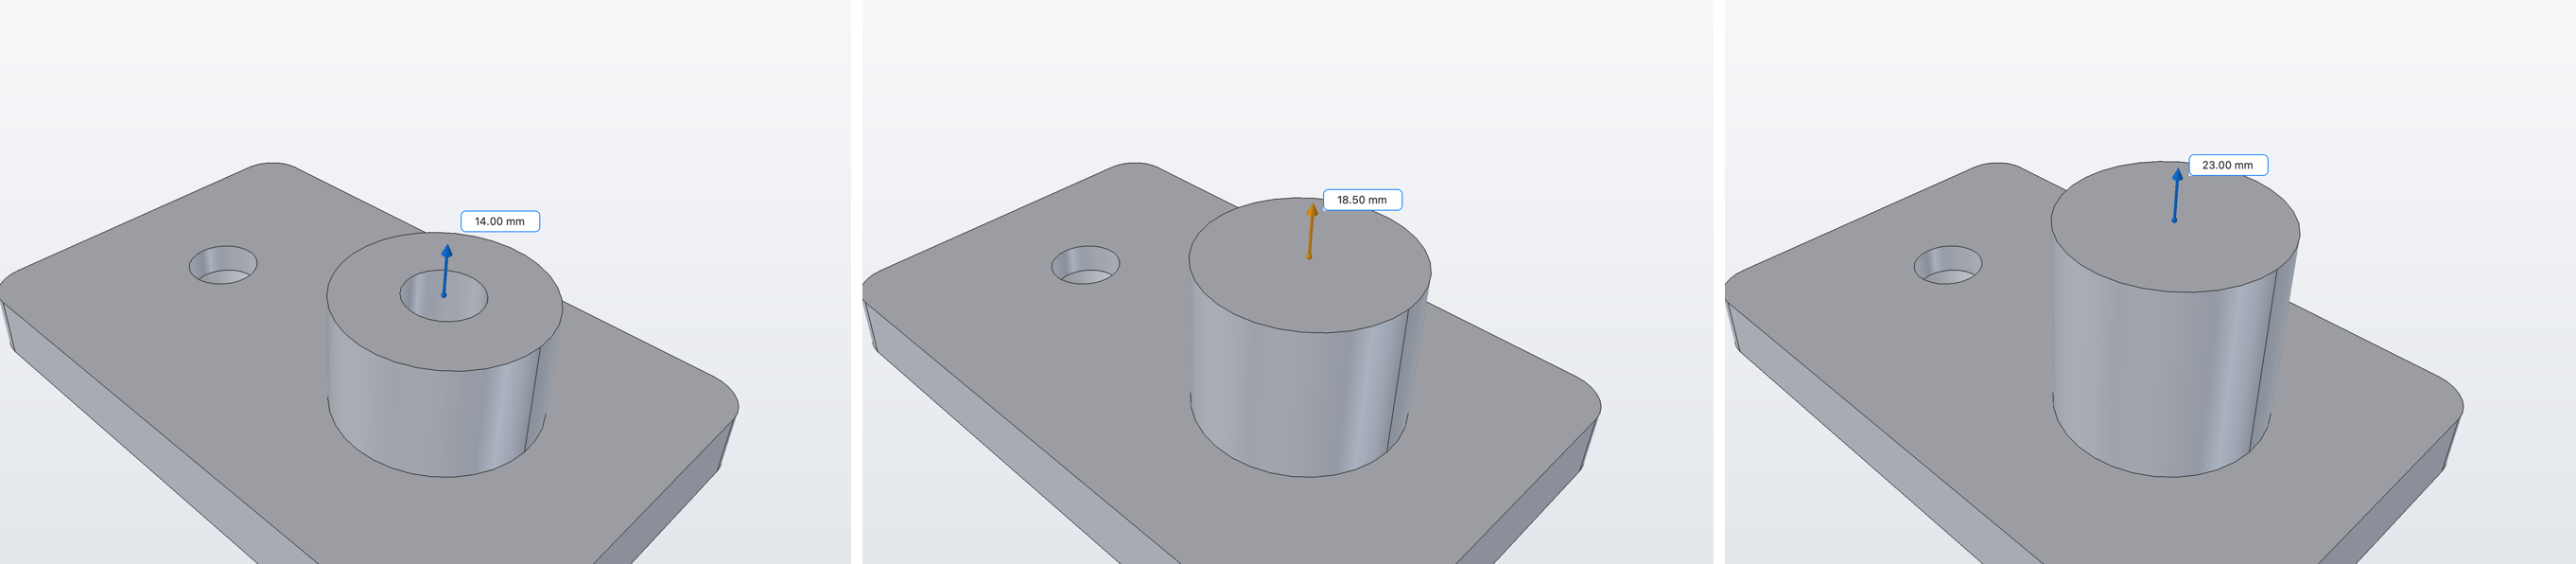
\includegraphics[width=\linewidth]{fig/mod14_spike.png}}{\fbox{mod14\_spike.png}}\\[2mm]
\IfFileExists{fig/mod14_spike_fc.png}{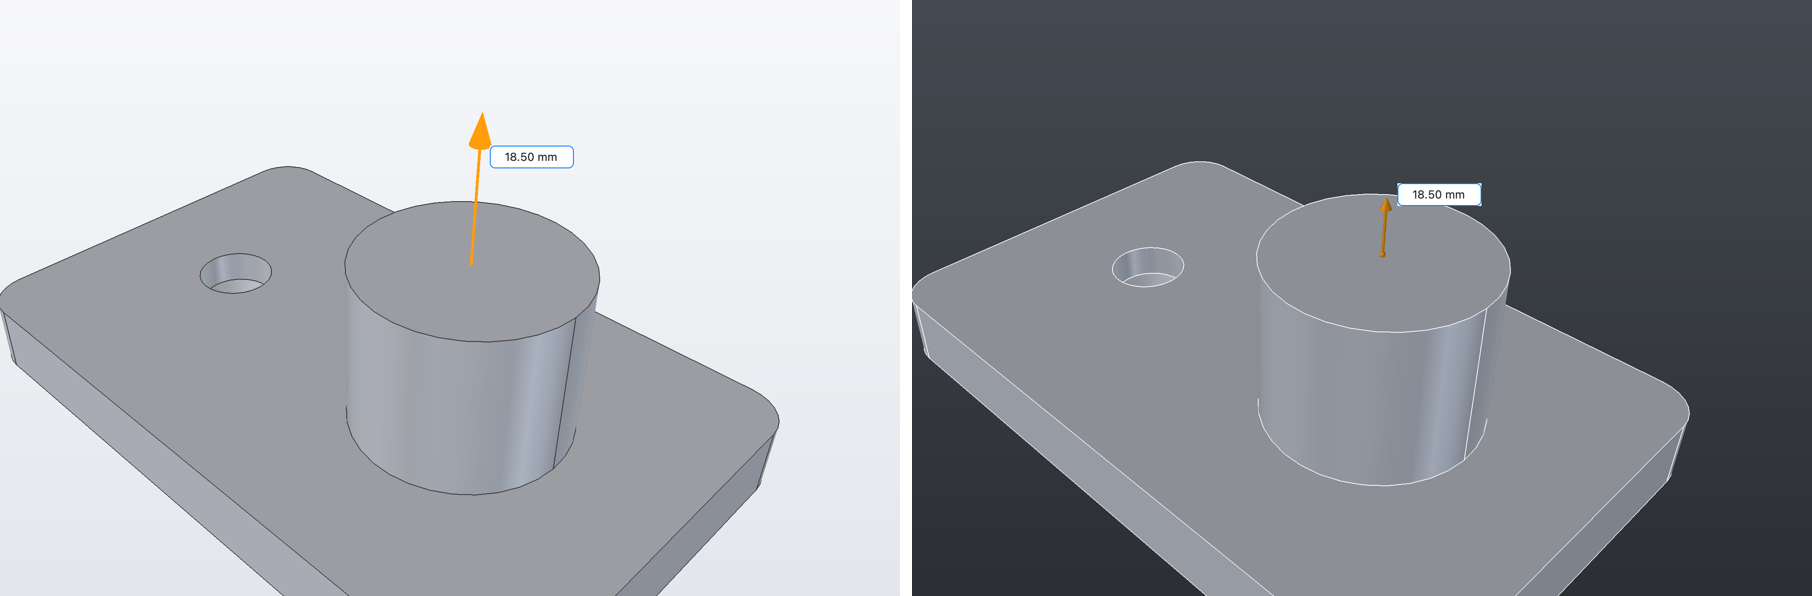
\includegraphics[width=0.66\linewidth]{fig/mod14_spike_fc.png}}{\fbox{mod14\_spike\_fc.png}}
\caption{The spike in this build (3D view saved with \code{saveImage}, the field painted over it; not a mock).
\emph{Top:} before, during and after the drag, pivy arrow. \emph{Bottom:} FreeCAD~1.1's own dragger driven from
Python, and the pivy arrow in dark mode. The value field is unstyled.}
\label{fig:mod14-spike}
\end{figure}

\textbf{Feasibility: Python only} for the first version. \code{[BW]} C++ is not needed; it would only become
useful to reuse \code{GizmoContainer} whole (its auto-scale and camera-facing logic, about 60 lines we redo in
Python), or if a navigation style turns out to claim the double-click.

%----------------------------------------------------------------------
\subsubsection*{2. Theory}

\paragraph{From a face to a parameter.} The double-click gives an object path and a face, e.g.
\code{Body.Fillet.Face5}; the Body shows its tip, so the face belongs to the tip's shape. FreeCAD's element map
traces it back: \code{getElementHistory(face, recursive=True)} lists every feature the face passed through, the last
being the one that made it (\S\ref{sec:uix12-plan}, tested). That feature and the face's role decide the handle:
\begin{center}
\small
\begin{tabularx}{\linewidth}{@{}p{3.6cm}p{4.4cm}X@{}}
\toprule
Feature and mode & Handle: base, direction $\hat u$ & Value from the drag $\Delta t$\\
\midrule
Pad, \code{Type} Length, one side & centre of the cap face; the resolved \code{Direction}, negated when \code{Reversed} & $L = L_0 + \Delta t$\\
Pad, \code{SideType} Symmetric (\code{Midplane} in older files) & both caps, $\pm\hat u$ & $L = L_0 + 2\Delta t$\\
Pad, Two sides & the cap on $+\hat u$ drives \code{Length}, on $-\hat u$ \code{Length2} & $L_i = L_{i,0} + \Delta t$\\
Pad along a custom direction, \code{AlongSketchNormal} on & as above & $L = L_0 + \Delta t\,(\hat u\cdot\hat n)$, $\hat n$ the sketch normal\\
Pocket (same types) & the pocket's floor, into the material & $D = D_0 + \Delta t$\\
Up to face, Up to first, Through all & no arrow; the field shows the type & ---\\
Hole, \code{DepthType} Dimension & top of the first hole (below a counterbore), $-\hat n$ & $D = D_0 + \Delta t$\\
Hole diameter & a point on the rim, radially out & $\varnothing = \varnothing_0 + 2\Delta t$\\
Fillet & mid-point of the first filleted edge, along an adjacent face away from the edge & $r = r_0 + \Delta t\tan(\alpha/2)$\\
\bottomrule
\end{tabularx}
\end{center}
The direction rule is the one FreeCAD~1.1's own pad arrow uses (in
\code{TaskExtrudeParameters::\allowbreak setGizmoPositions}).
Its arrow starts at the sketch and ends at the cap; ours starts at the face you double-clicked, as Fusion does,
because that is where you are looking.

\paragraph{Fillet geometry.} Let the two faces meet at the edge with interior angle $\alpha$ ($90^\circ$ for a box
corner). A fillet of radius $r$ touches both faces; its centre is on the bisector at $r/\sin(\alpha/2)$ from the
edge, and it meets each face along a line at
\[
  s = \frac{r}{\tan(\alpha/2)}
\]
from the edge. The arrow runs along one face from the old sharp edge to that line (figure~\ref{fig:mod14-states}),
so dragging it by $\Delta t$ changes the radius by $\Delta t\tan(\alpha/2)$; at $90^\circ$, one to one. FreeCAD~1.1
uses the same factor (\code{correction = 1/tan(angle/2)}, \file{TaskFilletParameters.cpp:255}). The edge and its
faces come from the fillet's base shape (\code{Fillet.Base}), since the result no longer has the sharp edge.

\paragraph{Following the pointer along the arrow.} The arrow is the line $a(t) = p_0 + t\,\hat u$. The pointer
defines the view ray $r(s) = r_0 + s\,\hat d$ (from the eye in perspective; from the near plane along the view
direction in orthographic). The value follows the point of the arrow's line closest to the ray: minimise
$\lVert p_0 + t\hat u - r_0 - s\hat d \rVert^2$ over $t$ and $s$. With $b = \hat u \cdot \hat d$ and
$w = p_0 - r_0$, the two conditions $w\cdot\hat u + t - b s = 0$ and $w\cdot\hat d + b t - s = 0$ give
\[
  t^{*} = \frac{(r_0 - p_0)\cdot(\hat u - b\,\hat d)}{1 - b^2},
  \qquad \Delta t = t^{*}(\text{pointer now}) - t^{*}(\text{at press}).
\]
Using the difference makes the grab point stick to the pointer. Coin's \code{SbLineProjector}, inside both
draggers, computes the same. When the arrow points almost at you ($1 - b^2 < \sin^2 8^\circ$) the result is
unstable; the arrow is then drawn faded and the drag falls back to vertical pointer motion times the size of a pixel
at $p_0$ (as the navigation pill's pan does). Orbiting a little restores it.

\begin{figure}[!htbp]
\centering
\begin{tikzpicture}[scale=1.0,>=Stealth]
  \coordinate (E) at (0,0.2);
  \coordinate (P0) at (5.2,-0.6);
  \draw[bwgrey,thick] (E) circle (0.08) node[left=3pt,black] {$r_0$ (eye)};
  \draw[->,thick,bworange] (E) -- (8.6,2.4) node[right] {view ray $r(s) = r_0 + s\hat d$};
  \draw[thick,bwblue] (5.2,-1.4) -- (5.2,3.0) node[above] {arrow line $a(t) = p_0 + t\hat u$};
  \fill[bwblue] (P0) circle (0.07) node[right] {$p_0$};
  \draw[->,very thick,bwblue] (P0) -- (5.2,0.4) node[right] {$\hat u$};
  \coordinate (A) at (5.2,1.62);
  \coordinate (R) at (5.75,1.67);
  \draw[dashed] (A) -- (R);
  \fill[bwblue] (A) circle (0.06) node[left] {$a(t^{*})$};
  \fill[bworange] (R) circle (0.06) node[below right] {$r(s^{*})$};
  \draw[->,bwgrey] (E) ++(0.9,0.2) -- ++(0.8,0.21) node[below] {$\hat d$};
  \draw[|<->|,bwgrey] (4.85,-0.6) -- (4.85,1.62) node[midway,left=2pt] {$t^{*}$};
\end{tikzpicture}
\caption{The arrow's value is the parameter $t^{*}$ of the point on its line nearest to the pointer's view ray.}
\label{fig:mod14-ray}
\end{figure}

\paragraph{Snapping.} The value snaps to the step $q$ shown in the command bar: $v = q\cdot\operatorname{round}(v/q)$,
so the field always shows round numbers. The default step follows the zoom as FreeCAD~1.1's arrows do:
$q = 10^{\lfloor \log_{10} \ell \rfloor}$, where $\ell$ is the model length under 1.5\,\% of the view; at a typical
zoom that is 1\,mm, zoomed in 0.1\,mm. \emph{Shift} divides it by ten, \emph{Grid} uses the sketch grid. The value
also snaps (within 6\,px on screen) to the heights of other planar faces along $\hat u$: for a face point $q_i$,
$t_i = (q_i - p_0)\cdot\hat u$, so a boss can be dragged level with another one. A snap holds until the pointer is
10\,px away (hysteresis), so it does not flicker. A length never goes below one step: a pad is not dragged through
zero into a pocket (question~2).

\paragraph{Keeping up with the pointer.} The pointer moves 60--120 times a second; one recompute of the spike's
chain takes about 20\,ms. So at most one recompute runs at a time, and the latest value wins: a move that arrives
during a recompute only replaces the pending value, and the next recompute starts when the last one ends. That gave
one recompute per move in the spike, about 45 updates a second. When recomputes get slow (a moving average above
80\,ms, question~6), the drag switches to a \emph{preview}: only the edited feature is recomputed (1.9\,ms for the
boss alone instead of 13.9\,ms) and shown semi-transparent, and the features after it catch up on release
\verify.

\paragraph{One undo step.} Press opens a transaction (\code{openTransaction("Drag Boss distance")}), release
commits it, \emph{Esc} aborts it and puts the value back. A typed value is its own transaction. The toast of
\eref{UIX-10} names the step: ``Boss distance 14 $\rightarrow$ 20 mm $\cdot$ Undo''.

\paragraph{Expressions.} A parameter driven by an expression shows no arrow (as in 1.1, \code{hasExpression}); the
field shows the expression and typing a number asks whether to replace it.

%----------------------------------------------------------------------
\subsubsection*{3. How it behaves}

\begin{enumerate}[nosep]
  \item \textbf{Idle.} Nothing is shown. A single click selects, as today.
  \item \textbf{Double-click a face} in the view: the arrow, the field and the command bar appear. Typing goes
        straight into the field. A feature's row in the Browser does the same with \emph{Alt}-double-click; a plain
        double-click there keeps opening the task dialog, as in stock FreeCAD (question~1).
  \item \textbf{Drag the arrow}, or type and press Enter. \emph{Tab} moves to the next value of the same feature
        (pad: distance $\rightarrow$ taper; hole: depth $\rightarrow$ diameter).
  \item \textbf{Leave} with \emph{Done}, Enter on an unchanged field, a click on empty space or another
        double-click. \emph{Esc} undoes what this edit did. \emph{Edit\ldots} opens the feature's task dialog,
        where FreeCAD's own arrows take over.
\end{enumerate}
A face that no supported feature made (a side face of a pad, an imported body) shows a short hint and the inspector
instead. The arrow and field are Heuretes FreeCAD widgets on the 3D view, like the navigation pill: a child
\code{QWidget} placed at the arrow tip from \code{getPointOnViewport} (device pixels from the bottom, converted),
with a \code{Gui::QuantitySpinBox} and \code{Gui.ExpressionBinding} for units and expressions. Preference:
Preferences $\rightarrow$ BruceWorx $\rightarrow$ \emph{On-canvas editing} (default on).

%----------------------------------------------------------------------
\subsubsection*{4. Build order and effort}

\begin{center}
\small
\begin{tabularx}{\linewidth}{@{}lXl@{}}
\toprule
\# & Step & Effort\\
\midrule
1 & Controller: double-click filter, face $\rightarrow$ feature $\rightarrow$ handle, enter/leave, Esc,
    transactions, one-at-a-time recompute & 1\,d\\
2 & Arrow: FreeCAD~1.1's \code{SoLinearDraggerContainer} by type name, auto-scale to the zoom, accent colours,
    \code{addDraggerCallback}; pivy \code{SoTranslate1Dragger} as fallback & 0.5\,d\\
3 & Value field and command bar on the view: units, expressions, typing, Tab, light and dark & 1\,d\\
4 & Pad and Pocket: all types and side modes of the table, with unit tests of the mapping & 1\,d\\
5 & Fillet radius (placement ported from \file{GizmoHelper.cpp}) and Hole depth and diameter & 1.5\,d\\
6 & Snapping: step, Shift, grid, face heights, hysteresis; the near-parallel fallback & 1\,d\\
7 & Preview mode for slow models & 1\,d\\
8 & Checklist on \code{LE-02001} and the test files, preference, write-up & 0.5\,d\\
\midrule
 & Total & 7.5\,d\\
\bottomrule
\end{tabularx}
\end{center}
\textbf{Risks.} pivy's dragger callbacks crash (avoided: FreeCAD's \code{addDraggerCallback}). Our scene-graph node
must be removed when the view or document closes (the navigation pill's lifetime handling applies). A face traced to
the wrong feature after an odd boolean would put the arrow on the wrong value; the command bar names the feature so
it is visible. Recompute times grow with the model: preview mode (step~7) is the answer, but needs checking on the
largest checklist file. No upstream conflict: all Python, no C++.

%----------------------------------------------------------------------
\paragraph{Your answers to the questions below (24 Oct).} All seven as recommended. 1: \textbf{double-click a face}
only, a single click stays plain selection; in the Browser a double-click keeps the task dialog and
\emph{Alt}-double-click starts on-canvas editing. 2: the drag \textbf{stops} at the smallest step (no Pad turned into a
Pocket). 3: \emph{Up to face} and \emph{Through all} show \textbf{no arrow}; \emph{Edit\ldots} changes the type. 4: the
arrow starts \textbf{on the face}. 5: the snap step \textbf{follows the zoom}, shown in the command bar, Shift for
finer. 6: preview above \textbf{80\,ms}, as a preference. 7: FreeCAD's task-panel arrows are \textbf{recoloured to the
accent}. Building started 24 Oct.

\subsubsection*{Questions before MOD-14 starts}

\begin{enumerate}
  \item \textbf{Gesture.} Double-click only, or also show the arrow when a single face of a feature is selected?
        And in the Browser: should a plain double-click on a feature row start on-canvas editing instead of the task
        dialog?\\
        \emph{Recommendation:} double-click a face only; a single click stays plain selection. In the Browser keep
        the task dialog and use \emph{Alt}-double-click for on-canvas editing.
  \item \textbf{Below zero.} Fusion's press-pull turns a pad into a cut when dragged through zero. Do the same, or
        stop at the smallest step?\\
        \emph{Recommendation:} stop; changing a Pad into a Pocket changes the feature type and breaks references.
  \item \textbf{Other pad types.} For \emph{Up to face} or \emph{Through all}, show no arrow (field shows the type),
        or switch the pad to a length when you drag?\\
        \emph{Recommendation:} no arrow; \emph{Edit\ldots} to change the type.
  \item \textbf{Where the arrow starts.} On the face you double-clicked (Fusion, the mock) or at the sketch, as
        FreeCAD~1.1's task-panel arrows do?\\
        \emph{Recommendation:} on the face.
  \item \textbf{Snap step.} Follow the zoom (1.1's arrows), or a fixed 1\,mm?\\
        \emph{Recommendation:} follow the zoom, shown in the command bar; Shift for finer.
  \item \textbf{Slow models.} Switch to preview above which recompute time?\\
        \emph{Recommendation:} 80\,ms, as a preference.
  \item \textbf{FreeCAD's own arrows.} Recolour the task-panel arrows to the accent (theme style parameters) so both
        look the same?\\
        \emph{Recommendation:} yes.
\end{enumerate}
